\begin{pastexam}[label={px:ccu-113-swa-04}]{中正資工所甲組 113 學年度 第 4 題}
（單選）

Given a fully parenthesized arithmetic expression provided below, please answer the following questions from Q4 to Q5.
\begin{center}
B $-$ E/(A$-$D) + E + C * D $-$ A * B
\end{center}

(3\%) Please find the expression tree and answer the level-order traversal of the expression tree. When operators have the same precedence, please evaluate them sequentially in the order presented within the expression. For instance, in the expression "a + b + c," calculate "a + b" first before combining the result with "c."
\begin{enumerate}[label=\Alph*.]
\item \texttt{- + + - * A B B / E * E - C D A D}
\item \texttt{+ - + - * E * B / A B C D E - A D}
\item \texttt{- + * - + A B B / E * E - C D A D}
\item \texttt{- + - + * A B / B E * E - C D A D}
\item None of the above
\end{enumerate}
\end{pastexam}

\begin{pastsoln}
答案是 E（None of the above）。 選項 C 是把 $E + C * D$ 先合起來的樹，和題目自己規定的計算順序不合，見下。

題目說式子是「fully parenthesized」，其實沒有完全加括號；題目也規定同級運算由左往右算（$a + b + c$ 先算 $a + b$）。
照這個規定和「\texttt{*}、\texttt{/} 先於 \texttt{+}、\texttt{-}」（資結書第~6.3.3~節）加上括號：頂層是
$B - [E/(A - D)] + E + [C * D] - [A * B]$ 四個同級運算，由左往右，
\[
\Bigl( \bigl( (B - E/(A - D)) + E \bigr) + C * D \Bigr) - A * B .
\]
運算式樹（資結書第~7.7~節）：最後算的運算子是根。
\begin{center}
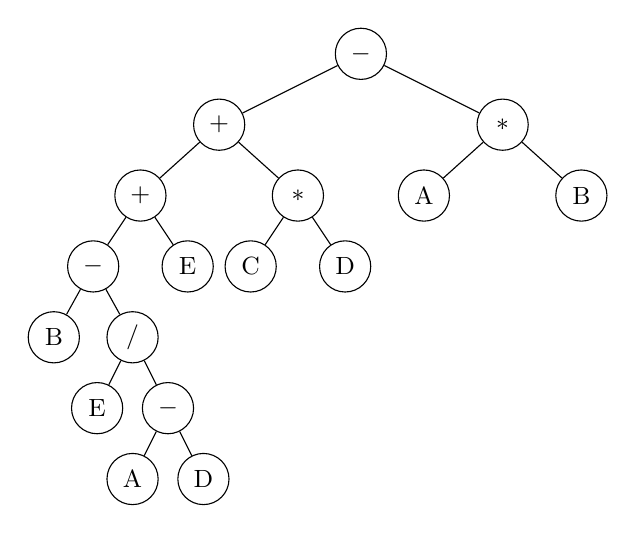
\begin{tikzpicture}[v/.style={circle,draw,minimum size=6.5mm,inner sep=0pt,font=\small},
  level distance=9mm, level 1/.style={sibling distance=36mm}, level 2/.style={sibling distance=20mm},
  level 3/.style={sibling distance=12mm}, level 4/.style={sibling distance=10mm}, level 5/.style={sibling distance=9mm}]
\node[v] {$-$}
  child {node[v] {$+$}
    child {node[v] {$+$}
      child {node[v] {$-$}
        child {node[v] {B}}
        child {node[v] {/} child {node[v] {E}} child {node[v] {$-$} child {node[v] {A}} child {node[v] {D}}}}}
      child {node[v] {E}}}
    child {node[v] {$*$} child {node[v] {C}} child {node[v] {D}}}}
  child {node[v] {$*$} child {node[v] {A}} child {node[v] {B}}};
\end{tikzpicture}
\end{center}
層序走訪（資結書第~7.3.2~節）一層一層由左往右：
\begin{center}
\begin{tabular}{cl}
\toprule
層 & 節點 \\
\midrule
0 & $-$ \\
1 & $+$\quad $*$ \\
2 & $+$\quad $*$\quad A\quad B \\
3 & $-$\quad E\quad C\quad D \\
4 & B\quad / \\
5 & E\quad $-$ \\
6 & A\quad D \\
\bottomrule
\end{tabular}
\end{center}
得 \texttt{- + * + * A B - E C D B / E - A D}，四個選項都不是，選 E。

逐項檢查：
\begin{itemize}
\item A：\texttt{- + + - * \ldots}，第 $1$ 層是兩個 \texttt{+}，表示根的右子樹也是加法，但最後減去的是 $A * B$，根的右子節點
是 \texttt{*}。 錯。
\item B：根是 \texttt{+}，但最後算的是減去 $A * B$，根應該是 \texttt{-}。 錯。
\item C：\texttt{- + * - + A B B / E * E - C D A D} 是樹
$\bigl((B - E/(A - D)) + (E + C * D)\bigr) - A * B$ 的層序，也就是先把 $E + C * D$ 算好再和前面相加。 數值上相同，但
違反題目「同級由左往右」的規定（等於先算了後面那個 \texttt{+}）。 錯。
\item D：第 $1$ 層是 \texttt{+ -}，根的右子節點成了 \texttt{-}，但根的右子樹是 $A * B$，應該是 \texttt{*}。 錯。
\item E：照題目的規定，正確的層序不在 A--D 裡。 對。
\end{itemize}
如果命題時把式子讀成 $(B - E/(A - D)) + (E + C * D) - A * B$，預期的答案會是 C；作答時可以在答案卷上寫出採用的
讀法。
\end{pastsoln}
